\begin{post}
	\postdata{Culinary adventures I.}{2011}{10}{22}{13}{54}{59}
	\begin{content}
One of the basic rules of blogging is: \textit{``Never start a post with} 'I don't know what to write'. \textit{If you don't know, then just \textbf{don't write anything}!''}. Sometimes that's easier said than done. You know, when you get used to blogging about your life and other peculiarities regularly, you miss it when there is nothing interesting going around. For me, blogging became some kind of relax, during which I still do something useful and refresh my mind and brain. Today, I really felt like blogging to take a break from all the pressure and stress about assignments and exams, however, the topic was nowhere to be found. And then it struck me --- food! I haven't told you about food here. And because it is quite an extensive topic, let's take it easy and slow.

Since there is no kitchen in the dorms, we are not able to cook for ourselves. That implies, that we have to ``eat out'' for both lunch and dinner. First choice we have to make is whether to go to the cafeteria or not. The KAIST cafeteria is located at the campus in the Union building, and for 3000KRW offers two kinds of meal (international and Korean) for lunch and one for dinner. They also have breakfast, but that is a typical Korean breakfast (i.e. rice, kimchi, soup, {\ldots}), which I am not able to process. The quality of the meals in the cafeteria is very unstable. Some meals, such as chicken curry, hamburger or japanese noodles are very good, but in other cases it is really not my kind of tea. From that reasons, I quite hesitate before I go to the cafeteria, because in most cases I pay for food that I 1) don't like and 2) won't finish. Not a good deal, right\ldots

The second choice is ``eating out out''. The neighborhood around our campus is quite restaurant-rich, so there is plenty of places to choose from. By now, we have established a bunch of places that we go into, and I will quickly introduce each one of these. Please note that in most cases I don't know the real name of the place, so I will refer to them using our nicknames.

\subsection{The regular place}
This place was discovered by Marc and it soon became our favorite place to eat. It is just a small room with a counter and a kitchen, where you order your food and get it packed in styrofoam boxes for take away. If you don't want to do take away, they have a room in the basement, where you can eat your meal. Simple, huh?

\begin{wrapfigure}[10]{R}{0.43\textwidth}
\vspace{-12pt}
\raggedleft\fbox{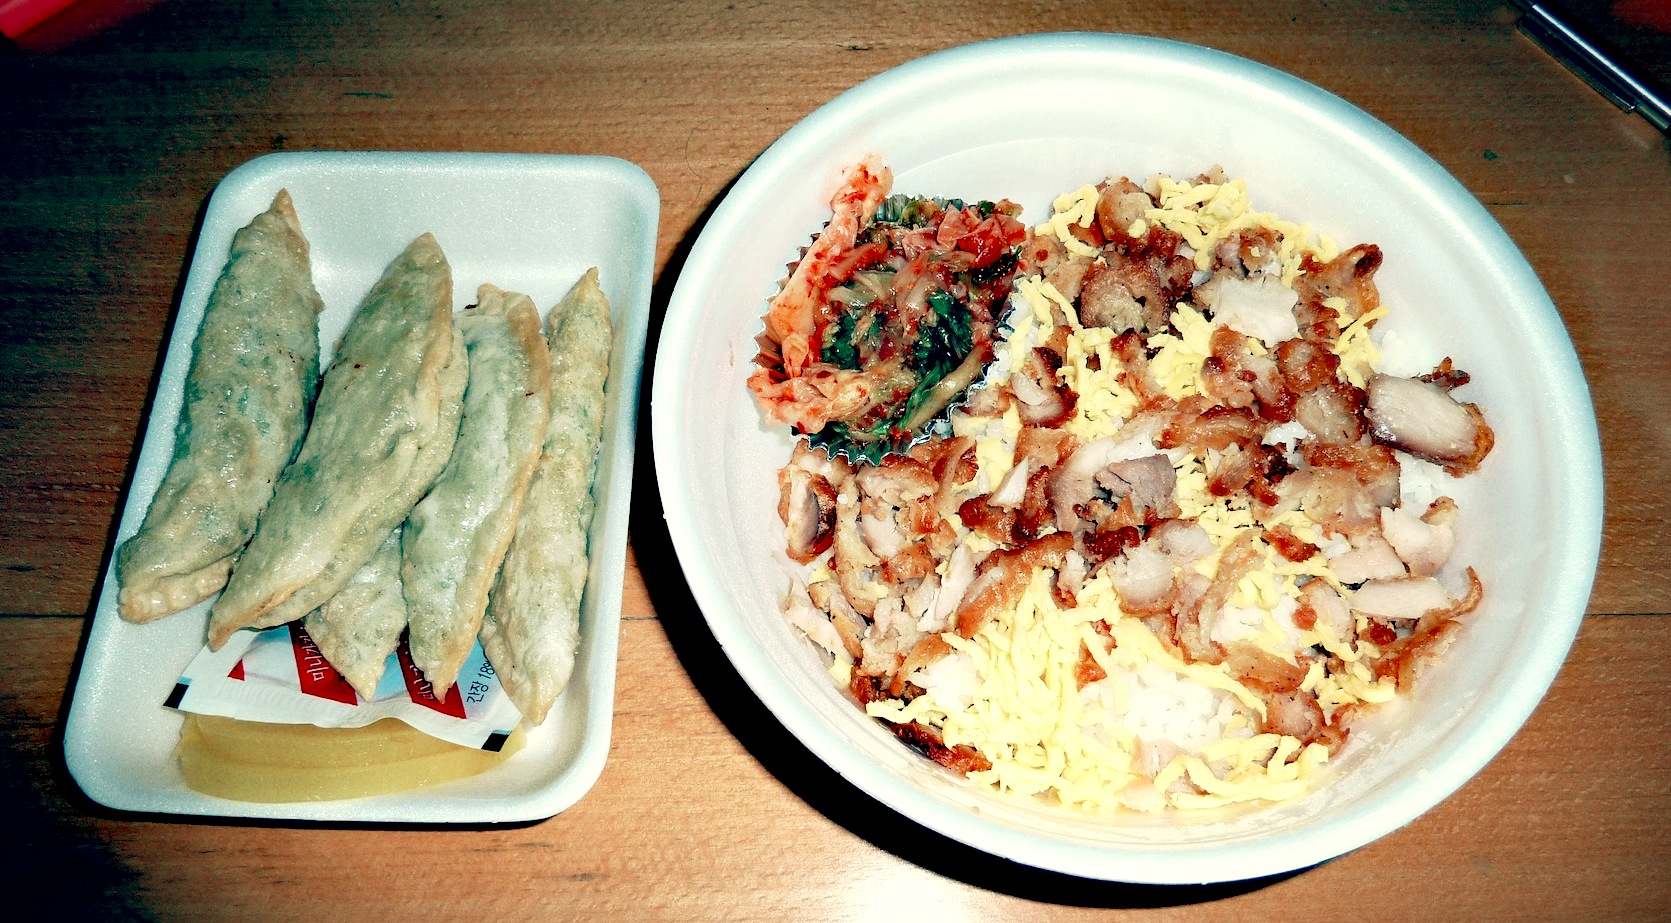
\includegraphics[height=8.5\baselineskip]{photos/10/22/p1000937.jpg}}
\vspace{-24pt}
\end{wrapfigure}There are two things that are perfect about this place --- it is fast and it is cheap. And it is also good.  Most meals are a combination of some meat (pork, chicken, hamburger patty, tuna) and rice, with kimchi and the yellow reddish as side dish. Our most favorite combination is {\H 빅치킨마요} and {\H 군만두} (big chicken mayo and kunmandu), which is rice + chicken + egg + kimchi + mayo and Korean dumplings, filled with a mixture of meat and vegetables. All this awesomeness for only 4400KRW (\EUR{2.7}).

Two weeks ago we have realized that we keep going to the same restaurants over and over again, which gets a little stereotypical. Therefore, Marc and I have decided that every Sunday evening, we will go to a new place in the neighborhood to try something different. I will try to keep you updated about our adventures, as well as describe other ``regular'' places, such as the curry place, the omelette place, the rice place, the chicken steak place, the dumpling guy or the japanese place. Stay tuned for another episode of CULINARY ADVENTURES with {\H 얀}!
\end{content}
\end{post}
